% Pagina iniziale
Dalla pagina iniziale del sito è possibile:

\begin{itemize}
\item Effettuare una ricerca (\S{8.1}),
\item Visualizzare la classifica con i migliori locali presenti su sito (\S{8.2}),
\item Filtrare i risultati (\S{8.3}) della classifica con i migliori locali tramite la zona geografica (\S{8.4}) ed il tipo di cucina (\S{8.5}).
\end{itemize}

\begin{figure}[H]
\centering
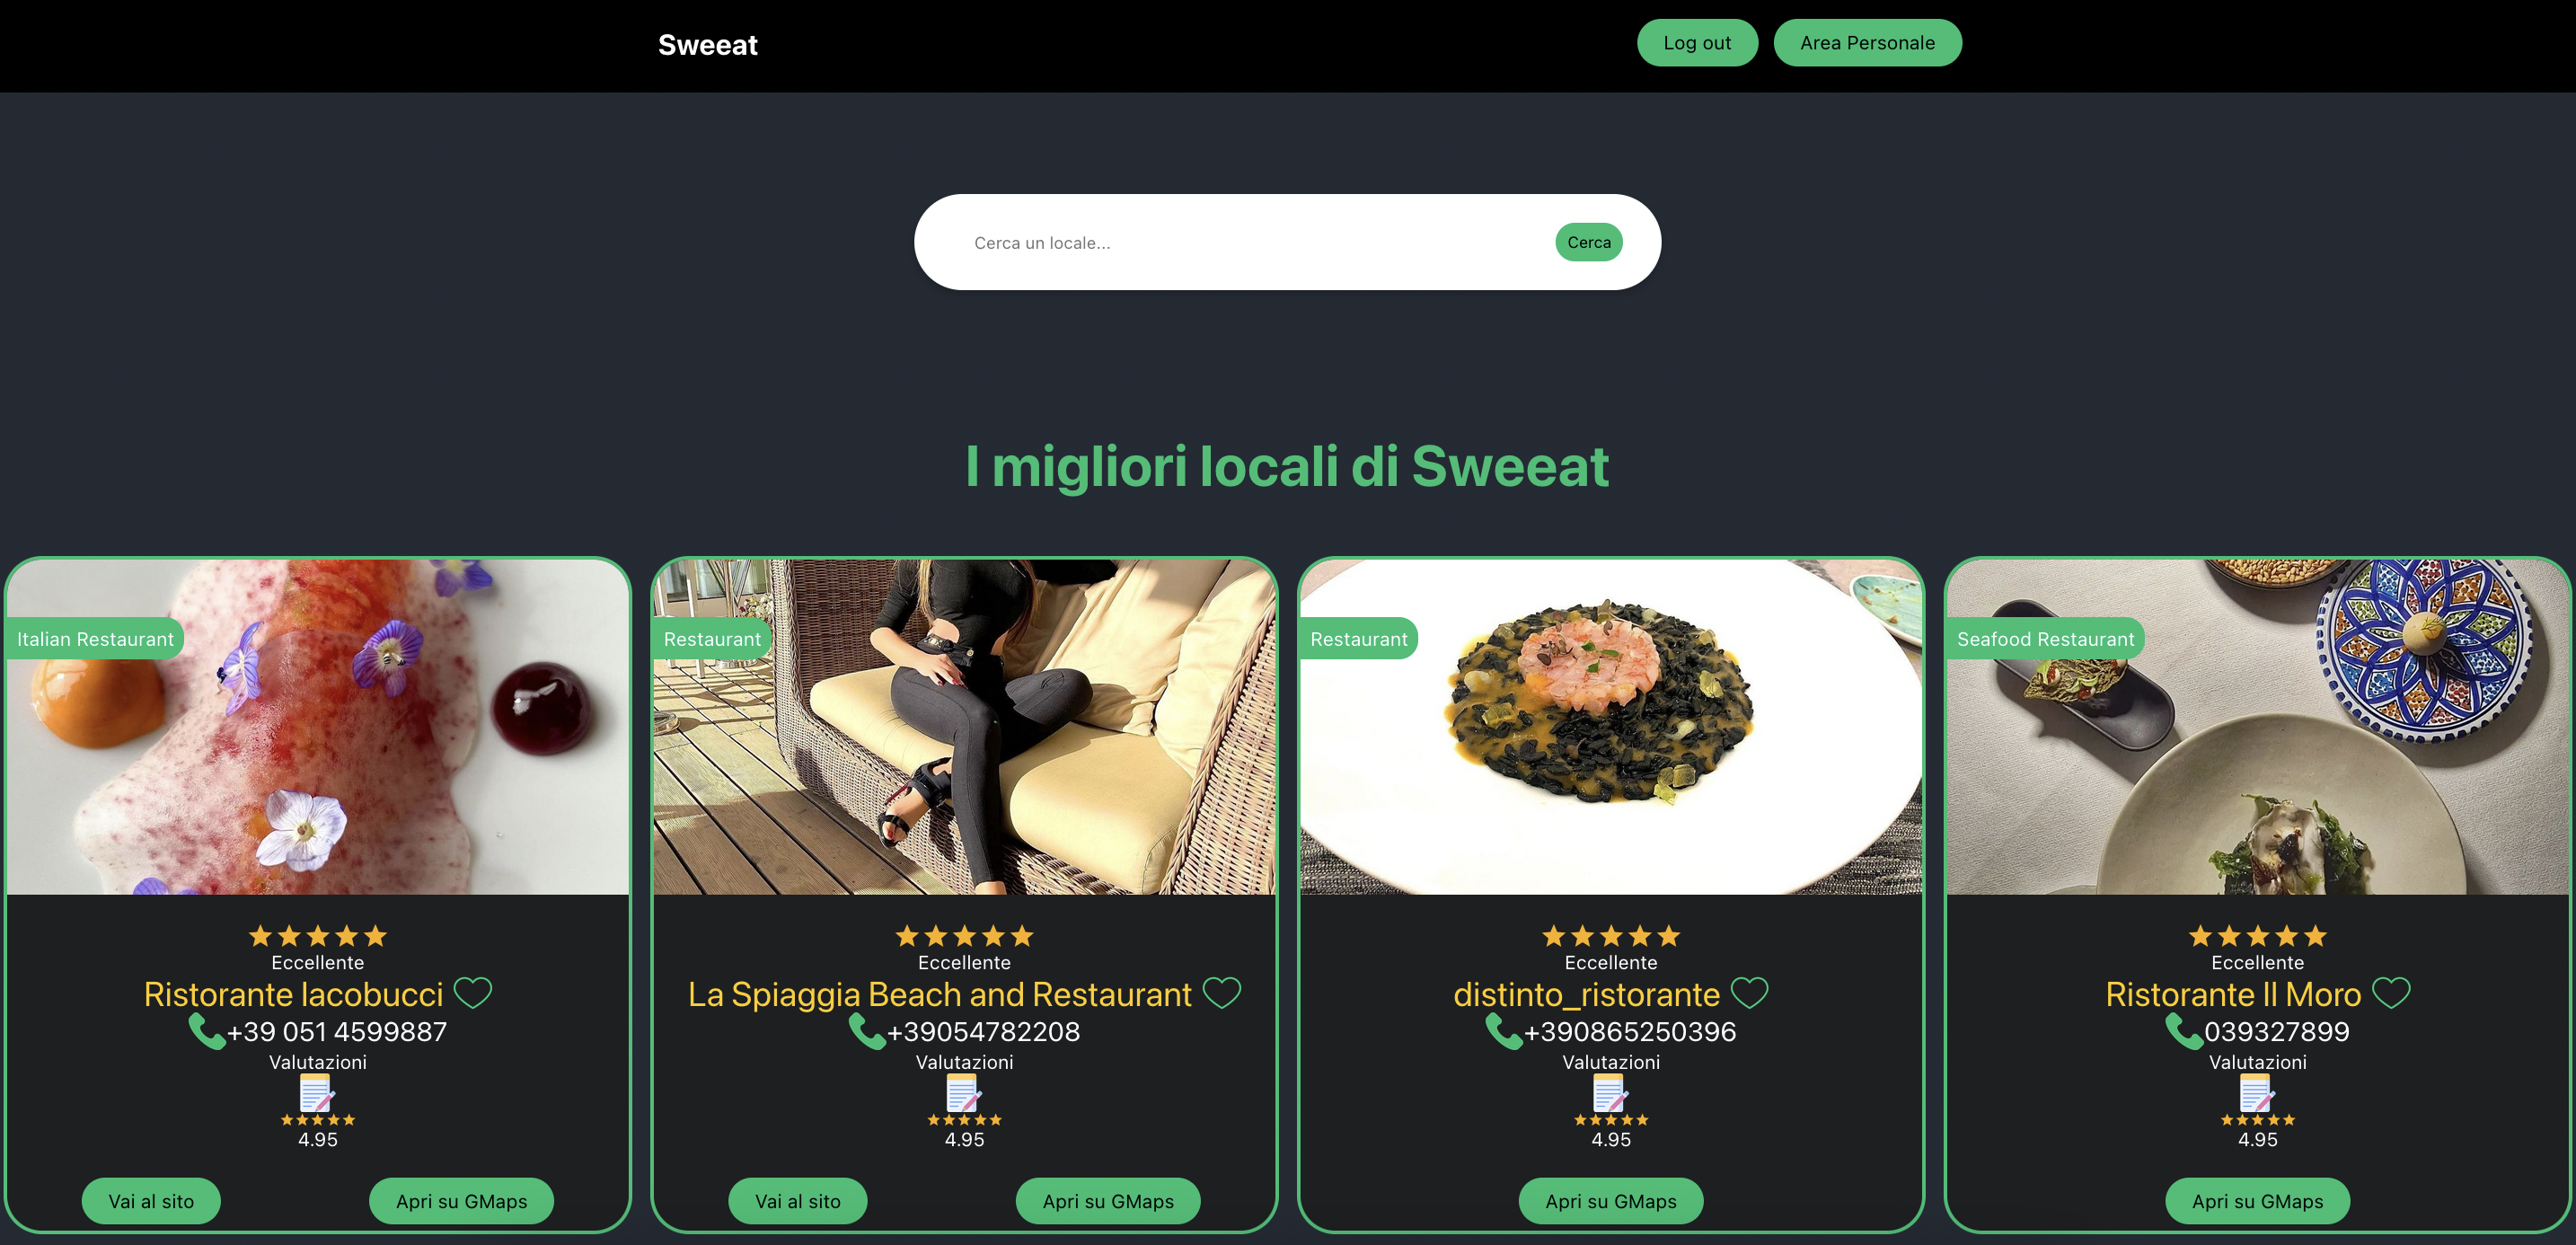
\includegraphics[scale=0.15]{./images/Homepage/Homepage.png} 
\caption{Homepage}
\end{figure}

\subsection{Ricerca}

Per effettuare una ricerca è necessario inserire il \textbf{nome del locale} cercato.

\begin{figure}[H]
\centering
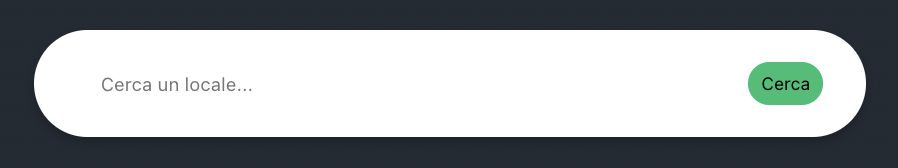
\includegraphics[scale=0.45]{./images/Homepage/Ricerca.png} 
\caption{Barra di ricerca nella Homepage}
\end{figure}

Quindi, va inserito il nome del locale da cercare e, per avviare la ricerca, è necessario cliccare su “\textbf{Cerca}”.

\begin{figure}[H]
\centering
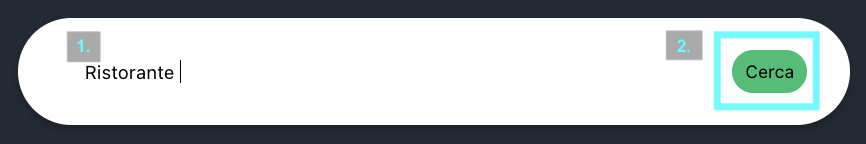
\includegraphics[scale=0.5]{./images/Homepage/Ricerca2.png} 
\caption{Inserimento dati ed avvio ricerca in Homepage}
\end{figure}

Una volta fatto ciò, verrà avviata la ricerca e l’utente verrà reindirizzato nella pagina dei risultati (\S{9}), la quale conterrà il risultato della ricerca (ossia, il locale cercato, dei locali alternativi o nessun locale).

\subsection{Visualizzare i migliori locali presenti su Sweeat}

Dalla pagina iniziale, oltre ad effettuare una ricerca, è possibile visualizzare i migliori locali presenti nella piattaforma ed interagire con essi.

La sezione dedicata ai migliori locali della piattaforma si trova sotto alla sezione contenente la barra di ricerca (sotto alla voce “I migliori locali di Sweeat”).

\begin{figure}[H]
\centering
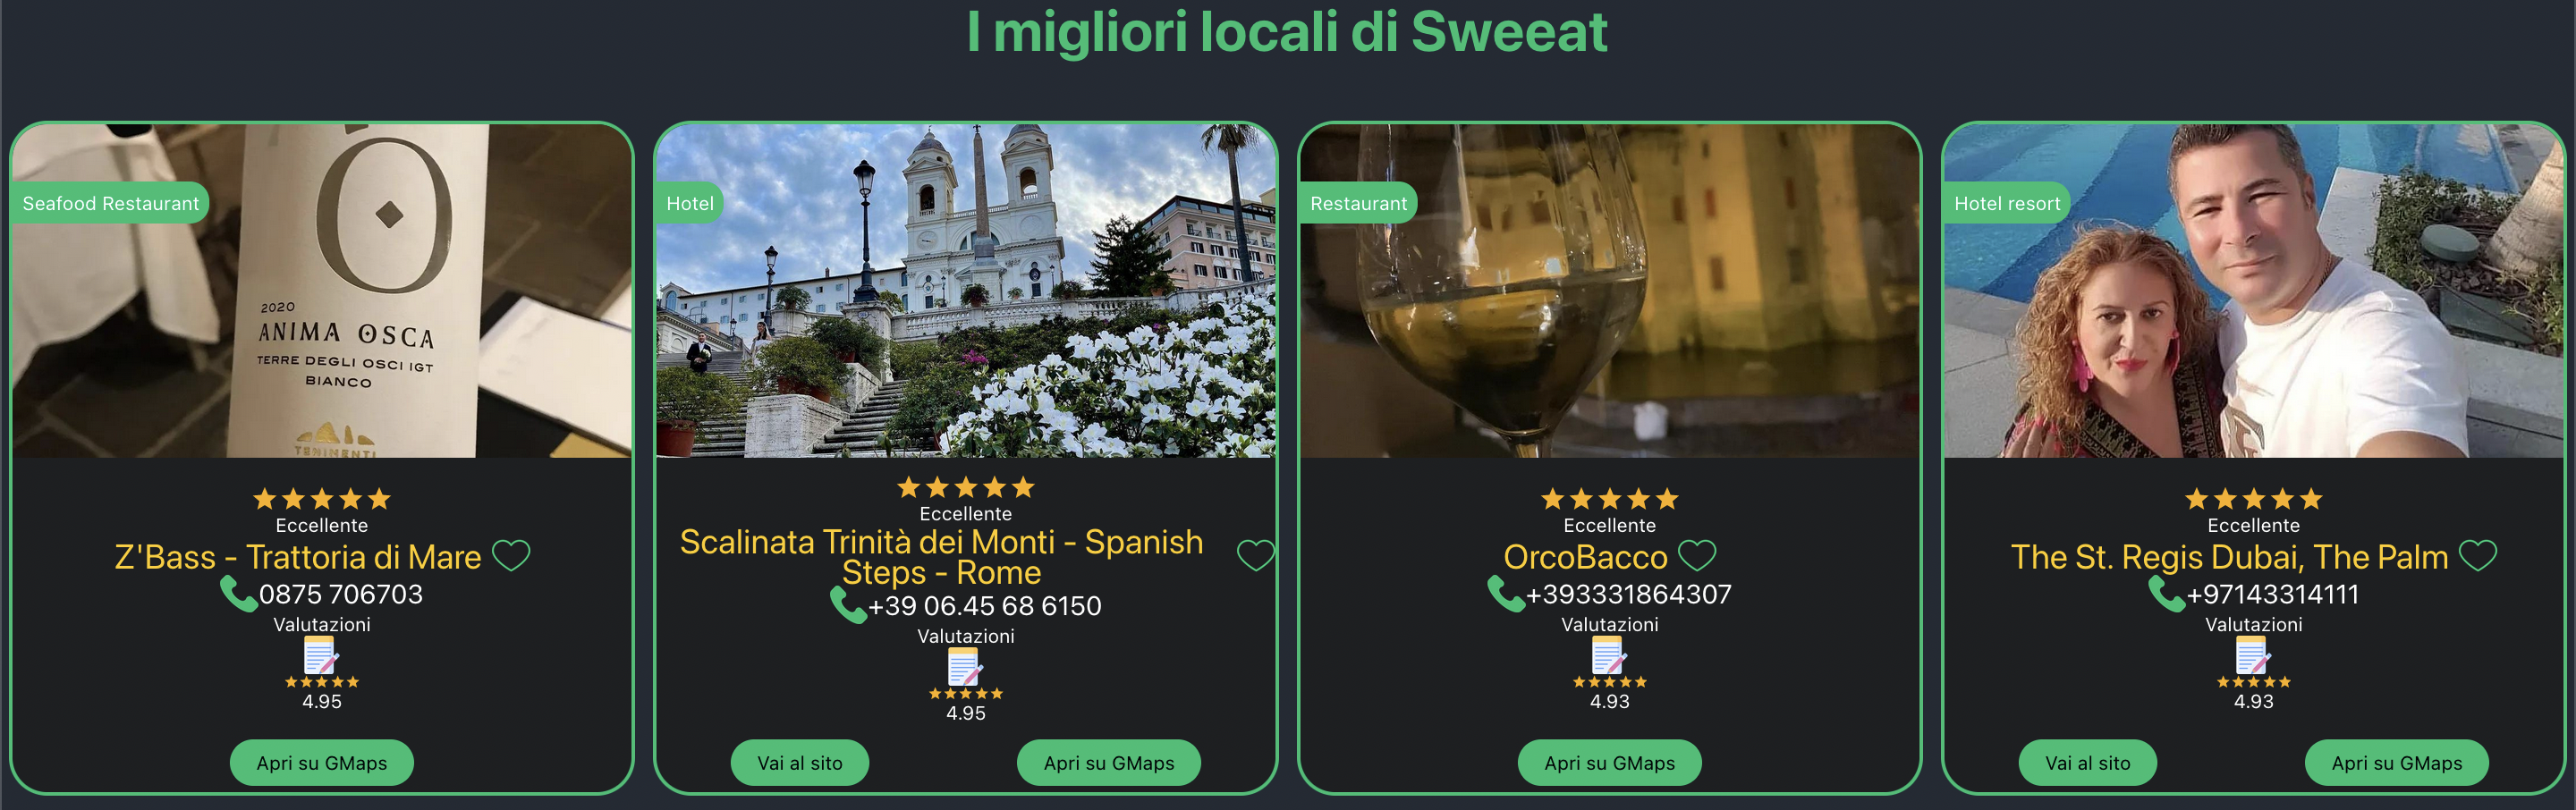
\includegraphics[scale=0.3]{./images/Homepage/MiglioriLocali.png} 
\caption{Inserimento dati ed avvio ricerca in Homepage}
\end{figure}

Per ciascun locale è possibile visualizzare le seguenti informazioni:

\begin{itemize}
\item Nome locale,
\item Valutazione complessiva,
\item Numero di telefono (opzionale),
\item Categoria,
\item Immagine di copertina,
\item Valutazione(*) per:
\begin{itemize}
\item Foto,
\item Testo,
\item Emoticons,
\end{itemize}
\item Link al sito web,
\item Link alla posizione del locale su Google Maps,
\item Possibilità di aggiungere o rimuovere il locale alla lista dei preferiti.
\end{itemize}

\begin{figure}[H]
\centering
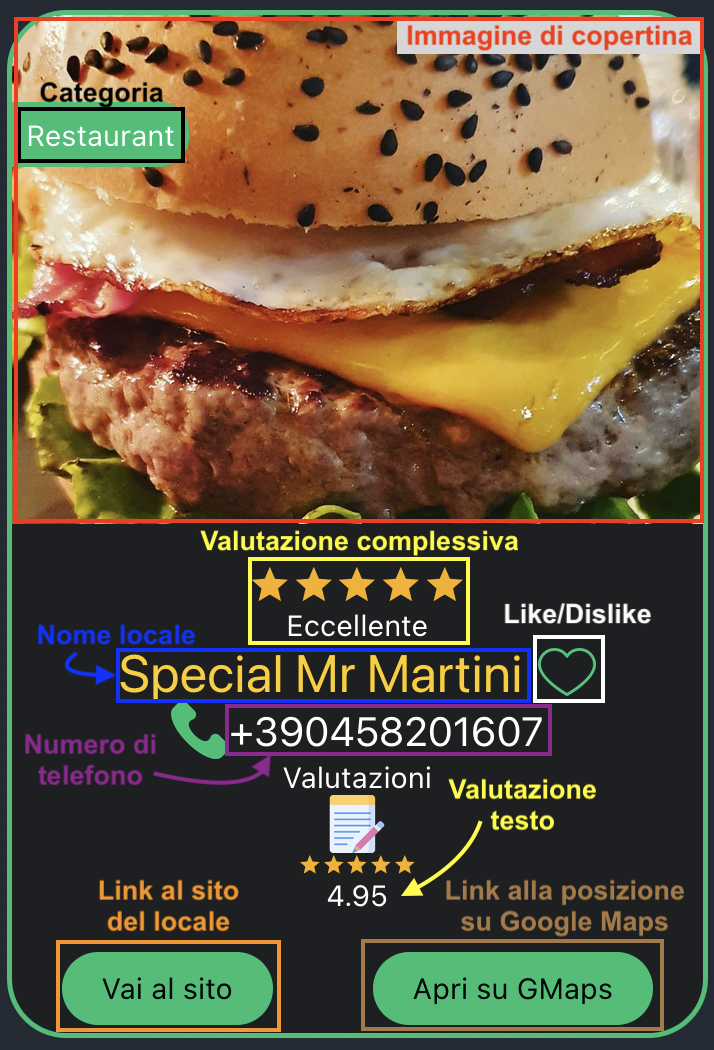
\includegraphics[scale=0.4]{./images/Homepage/Card.png} 
\caption{Card Locale in Homepage}
\end{figure}

(*) Per conoscere il significato delle valutazioni, consulta il paragrafo \S{9.2.1}. \\

La classifica dei migliori locali ha diverse pagine e per scorrerle è necessario cliccare su uno dei numeri presenti nella parte inferiore della pagina.

\begin{figure}[H]
\centering
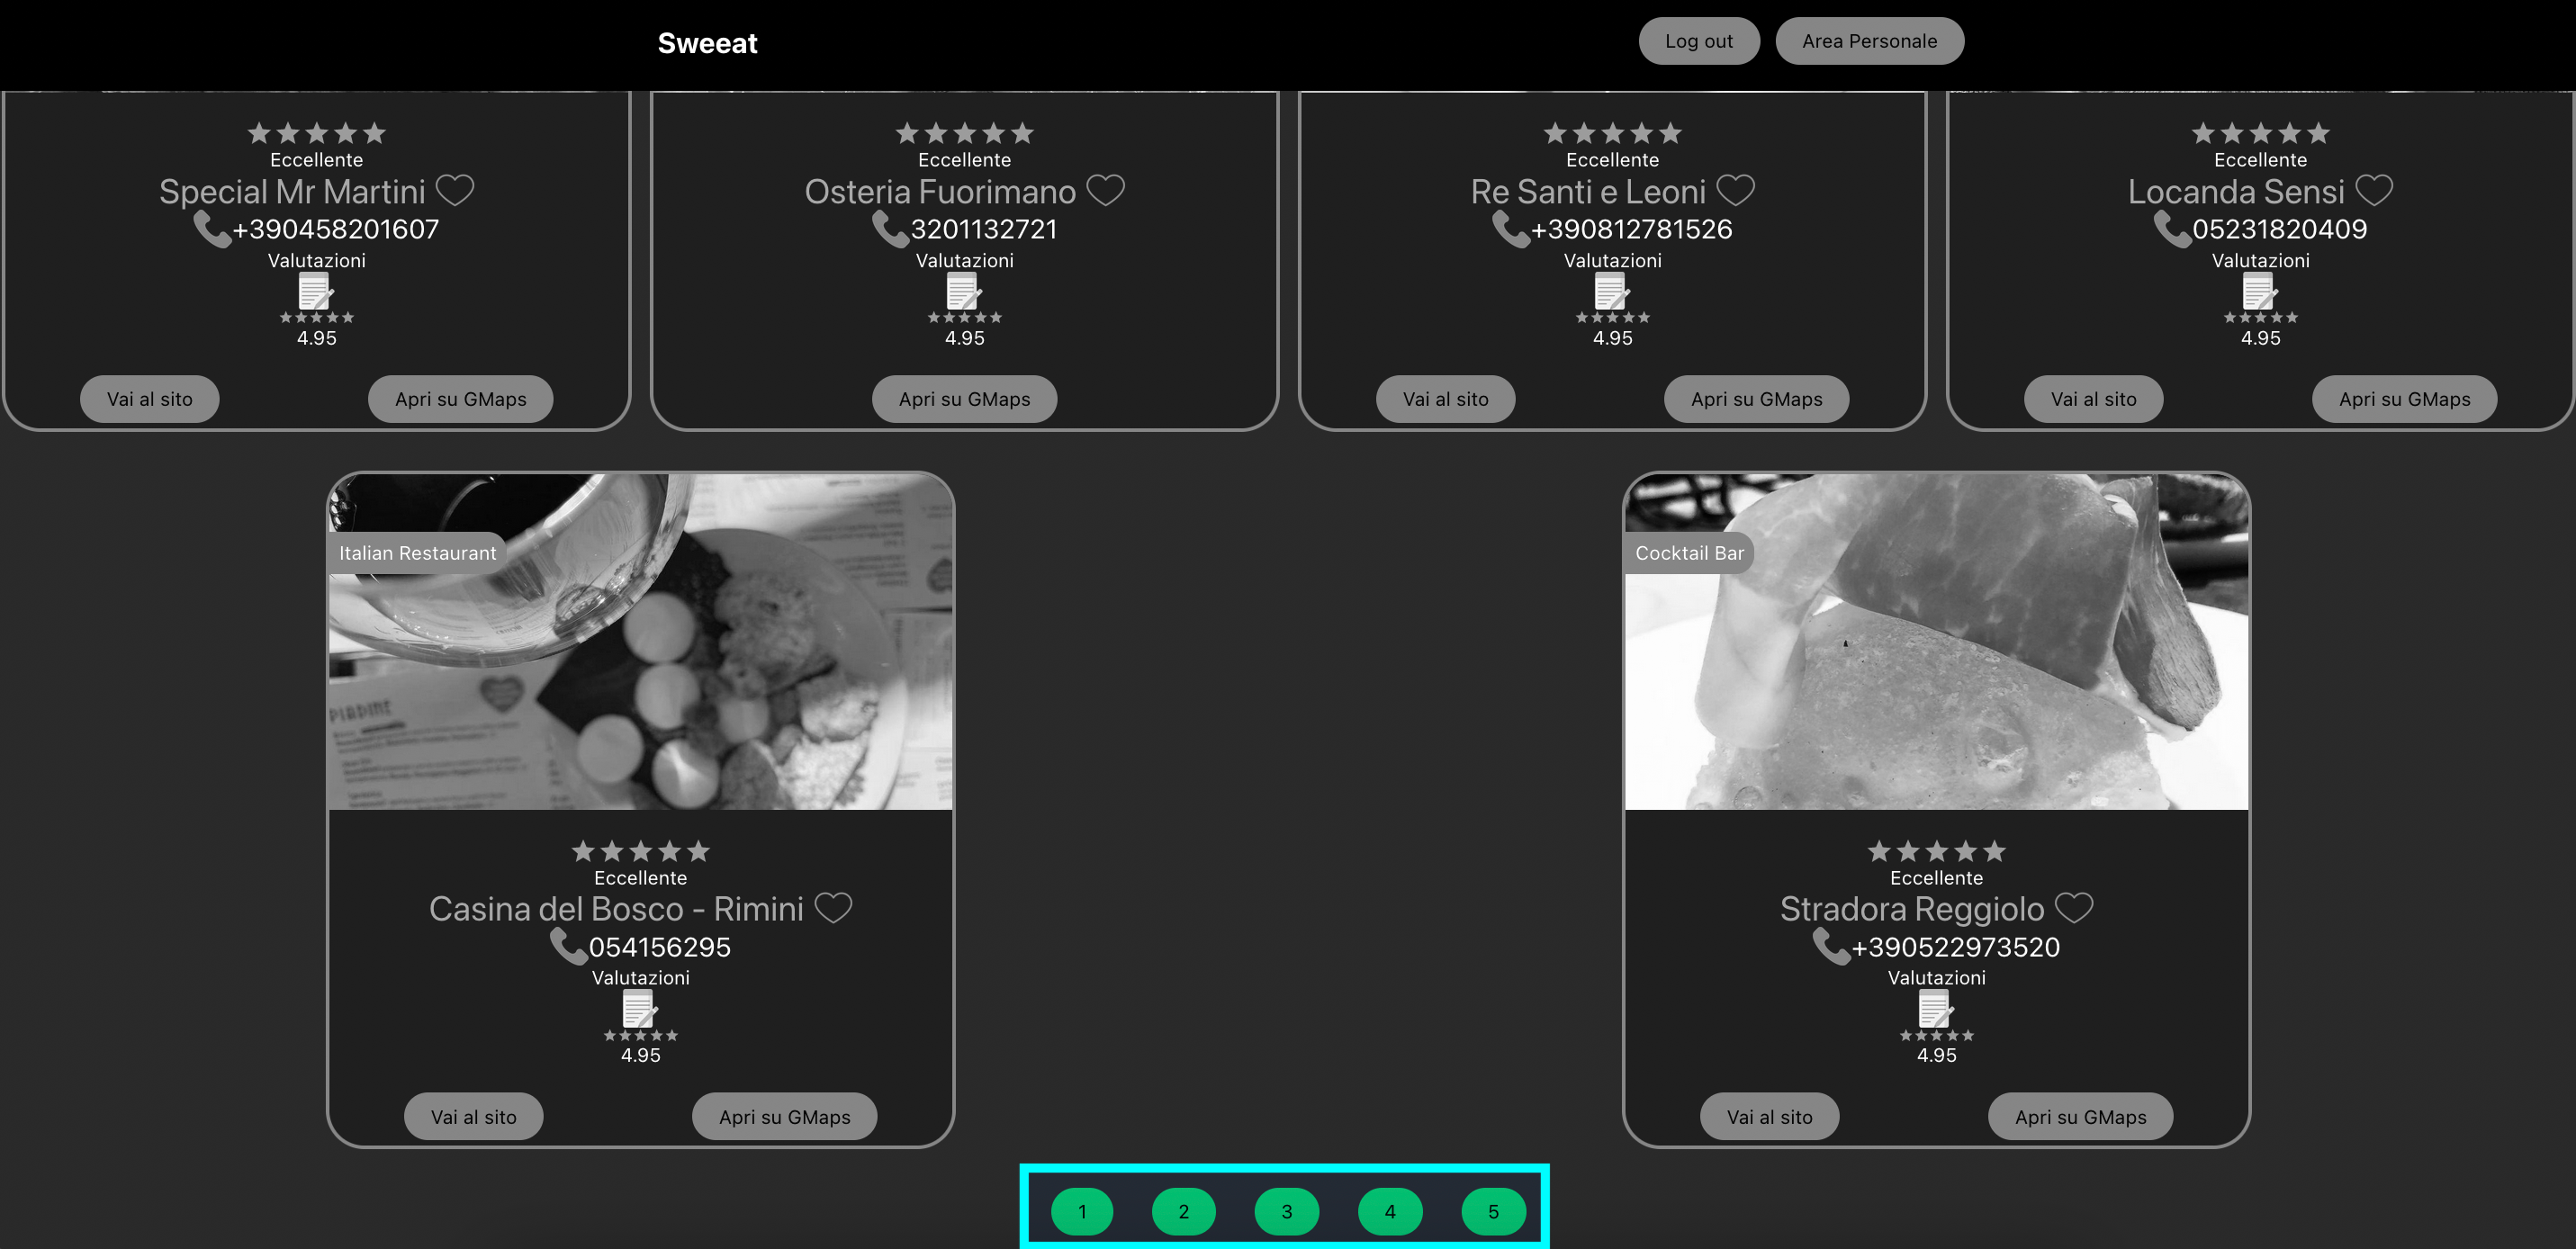
\includegraphics[scale=0.15]{./images/Homepage/Pagine.png} 
\caption{Visualizza altri migliori locali in Homepage}
\end{figure}

Inoltre, cliccando sul nome del locale all’utente verrà mostrata la \textbf{Pagina di dettaglio locale} (\S{10}) la quale, oltre al nome stesso del locale e le informazioni di base appena descritte, conterrà i contenuti multimediali relativi a quel locale pubblicati su Instagram ed utilizzati per realizzare la WebApp.

\subsection{Filtrare i risultati}

Al fine di ottenere una lista di risultati personalizzati in base all’interesse dell’utente, è possibile applicare dei filtri sulla classifica.

Attualmente, Sweeat offre i seguenti filtri:

\begin{itemize}
\item Per zona geografica (con possibilità di impostare il raggio di distanza dalla località impostata),
\item Per tipo di cucina.
\end{itemize}

L’utente può impostare la zona geografica d’interesse inserendo il nome della città nella casella di testo a sinistra (la quale darà anche dei suggerimenti per facilitare l'utente). Inoltre, è possibile ottenere maggiori risultati impostare anche il raggio (espresso in chilometri) dalla città scelta. Analogamente, è possibile digirtare il nome del tipo di cucina d’interesse nella casella di testo più a destra.

\begin{figure}[H]
\centering
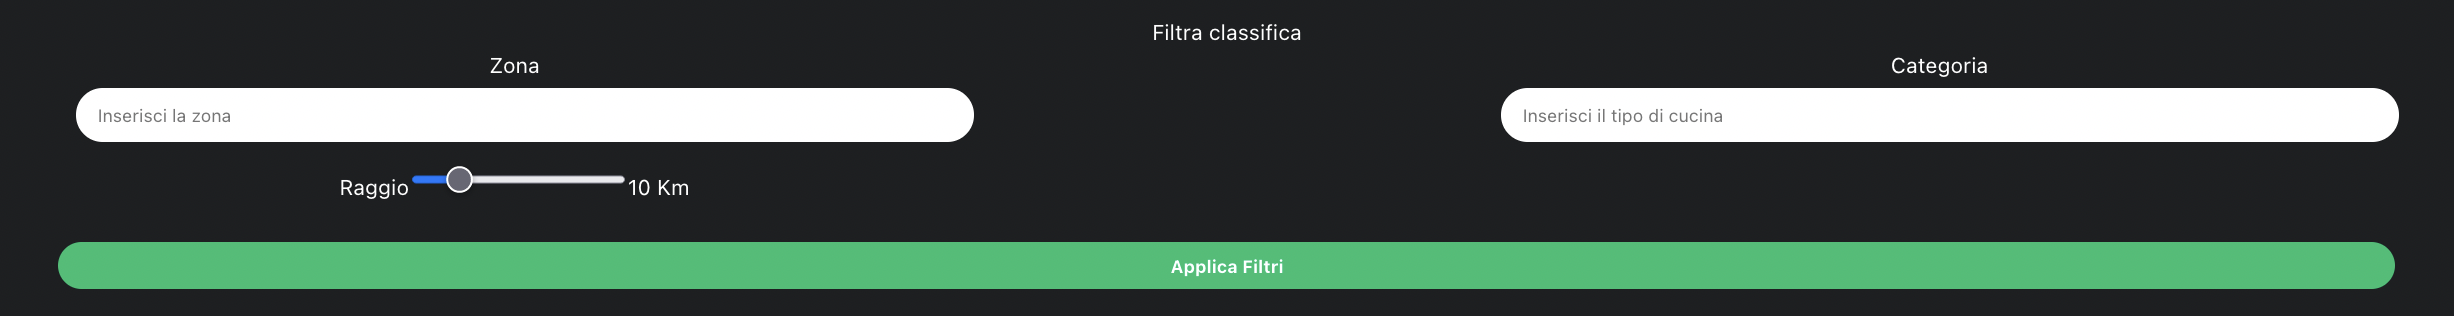
\includegraphics[scale=0.3]{./images/Homepage/Filtri.png} 
\caption{Filtrare i risultatati}
\end{figure}

\subsection{Filtrare per zona geografica}

È possibile filtrare la classifica dei migliori locali presenti nella piattaforma inserendo il nome della città di interesse:

\begin{figure}[H]
\centering
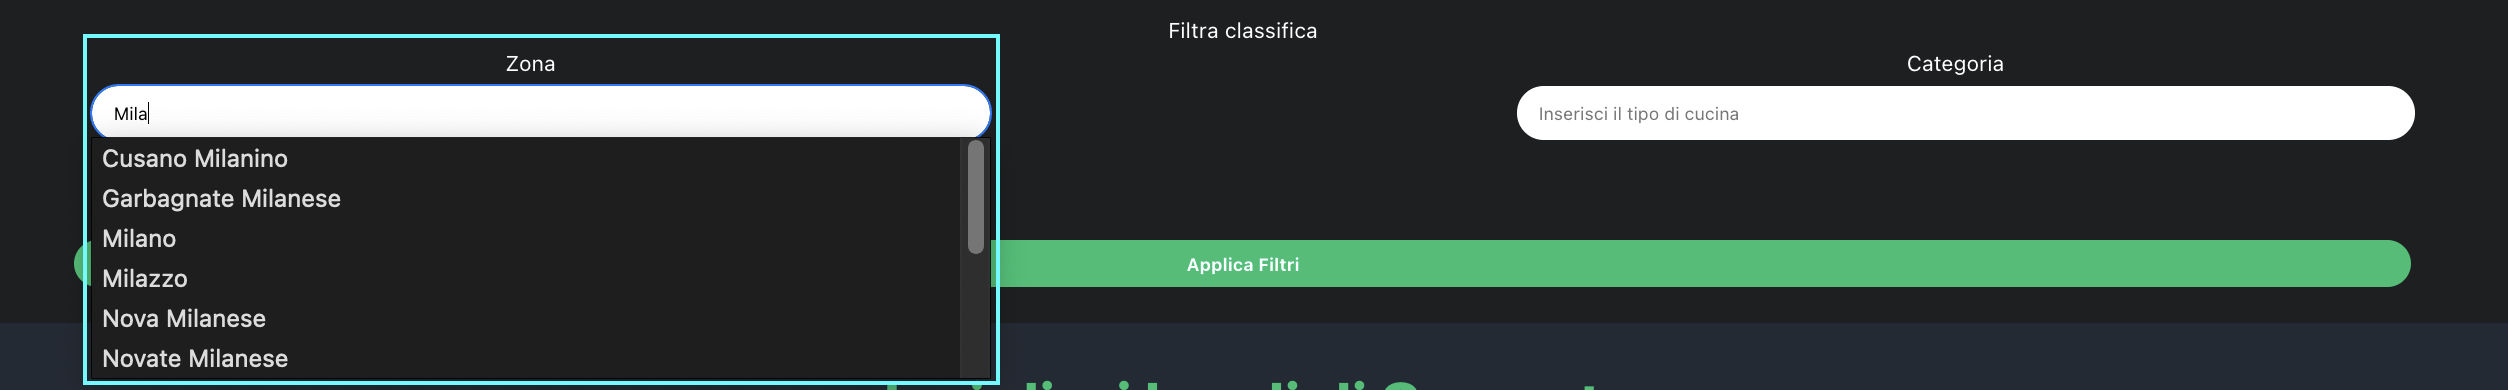
\includegraphics[scale=0.2]{./images/Homepage/FiltriZona.png} 
\caption{Filtrare i risultatati per zona geografica}
\end{figure}

Per filtrare per zona è necessario inserire la città nella casella di testo; la piattaforma aiuterà l'utente nell'inserimento con dei suggerimenti delle città presenti a sistema.

C'è la possibilità di impostare anche un raggio dalla città inserita nella casella di testo, al fine di ottenere una lista di risultati più esaustiva.

\begin{figure}[H]
\centering

\includegraphics[scale=0.4]{./images/Homepage/Raggio.png} 
\caption{Filtrare i risultatati per zona geografica e raggio}
\end{figure}

\subsection{Filtrare per tipo di cucina}

Oltre alla zona, è possibile filtrare per tipo di cucina: il funzionamento è analogo al filtro per zona geografica, basterà inserire il tipo di cucina nel campo di testo (anche qui, la piattaforma darà dei suggerimenti all'utente per semplificare l'operazione).

\begin{figure}[H]
\centering
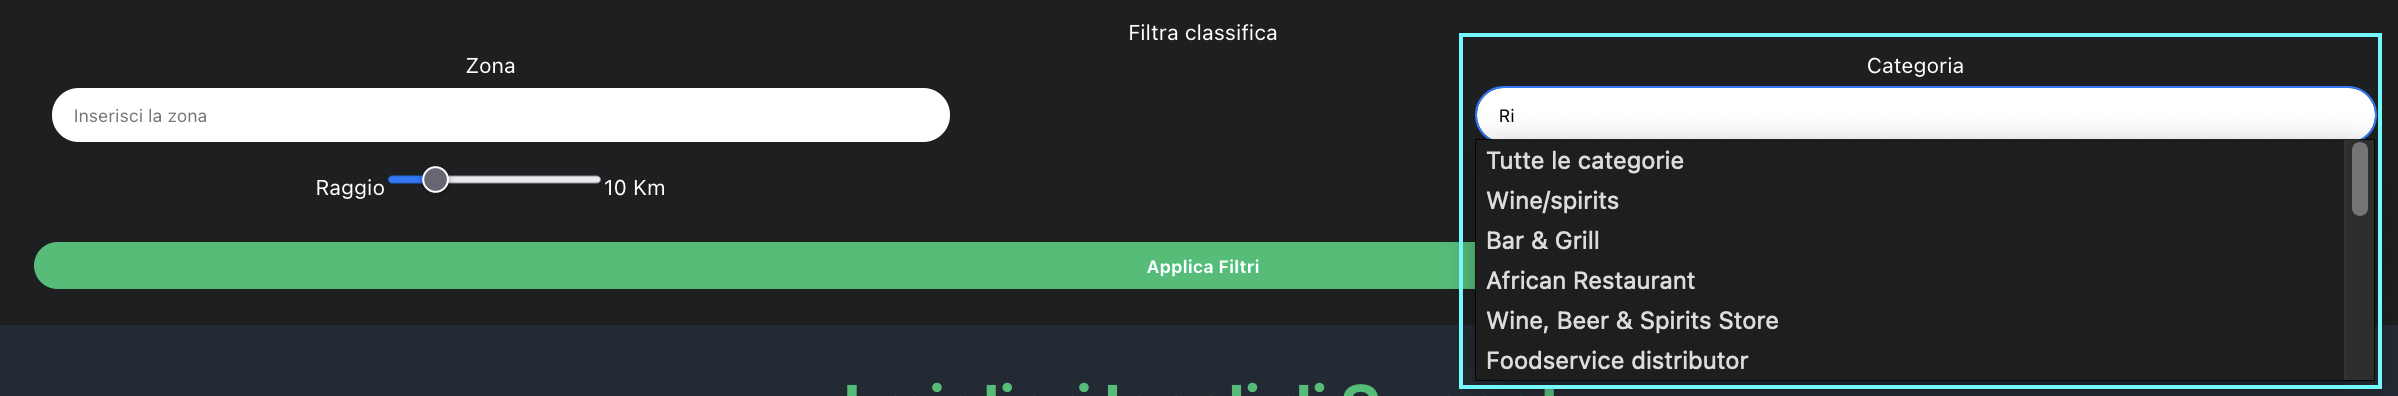
\includegraphics[scale=0.4]{./images/Homepage/FiltriCucina.png} 
\caption{Filtrare i risultatati per tipo di cucina}
\end{figure}

\subsection{Applicare i filtri}

Una volta impostati i filtri, affinché l’utente possa ottenere la lista con i risultati personalizzati in base alle sue scelte, dovrà cliccare sul bottone “\textbf{Applica Filtri}”.

\begin{figure}[H]
\centering
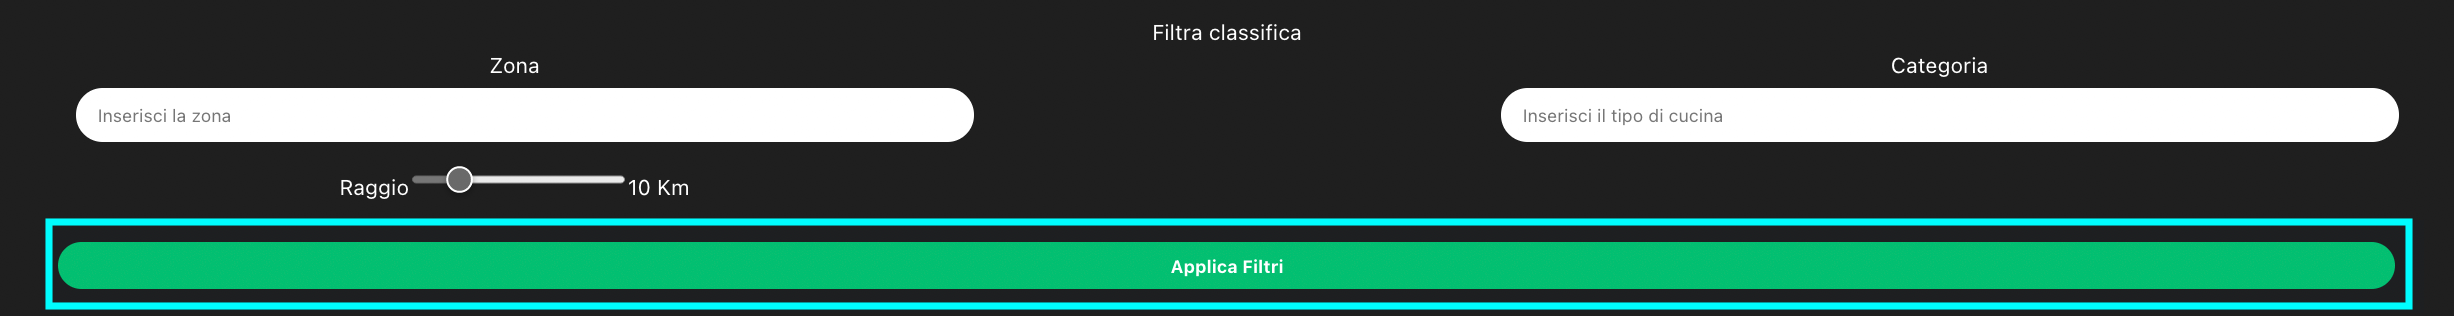
\includegraphics[scale=0.15]{./images/Homepage/ApplicaFiltri.png} 
\caption{Come applicare i filtri i risultati}
\end{figure}